\documentclass[12pt,a4paper]{article}
\usepackage{cmap} % Makes the PDF copiable. See http://tex.stackexchange.com/a/64198/25761
\usepackage[T1]{fontenc}
\usepackage[brazil]{babel}
\usepackage[utf8]{inputenc}
\usepackage{amsmath}
\usepackage{amsfonts}
\usepackage{amssymb}
\usepackage{amsthm}
\usepackage[usenames,svgnames,dvipsnames]{xcolor}
\usepackage{hyperref}
\usepackage{multicol}
\usepackage{graphicx}
\usepackage[top=2cm, bottom=2cm, left=2cm, right=2cm]{geometry}
\usepackage{cancel}

\hypersetup{
    colorlinks = true,
    allcolors = {blue}
}

% TODO: Consider using exsheets
% http://linorg.usp.br/CTAN/macros/latex/contrib/exsheets/exsheets_en.pdf
%
% http://ctan.org/tex-archive/macros/latex/contrib/exercise/
% Options: answerdelayed,lastexercise,noanswer
\usepackage[answerdelayed,lastexercise]{exercise}

\addto\captionsbrazil{%
\def\listexercisename{Lista de exerc\'icios}%
\def\ExerciseName{Exerc\'icio}%
\def\AnswerName{Solu\c{c}\~ao do exerc\'icio}%
\def\ExerciseListName{Ex.}%
\def\AnswerListName{Solu\c{c}\~ao}%
\def\ExePartName{Parte}%
\def\ArticleOf{de\ }%
}

\renewcommand{\ExerciseHeaderTitle}{(\ExerciseTitle)\ }
\renewcommand{\ExerciseListHeader}{%\ExerciseHeaderDifficulty%
\textbf{%\ExerciseListName\
\ExerciseHeaderNB.\ %
%\ --- \
\ExerciseHeaderTitle}%
%\ExerciseHeaderOrigin
\ignorespaces}
\renewcommand{\AnswerListHeader}{\textbf{\ExerciseHeaderNB.\ (\AnswerListName)\ }}

\newcommand*\sen{\operatorname{sen}}
\newcommand*\dom[1]{\operatorname{Dom}\left(#1\right)}

\renewcommand{\theenumi}{\alph{enumi}}
\renewcommand\labelenumi{(\theenumi) }

\newcommand*\tipo{Prova I}
\newcommand*\turma{NEXM241-D}
\newcommand*\disciplina{CDI1001}
\newcommand*\eu{Helder G. G. de Lima}
\newcommand*\data{17/04/2024}

\author{\eu}
\title{\tipo - \disciplina}
\date{\data}

\begin{document}
\thispagestyle{empty}
\newgeometry{margin=2cm,bottom=0.5cm}
\begin{center}

\includegraphics[width=9.0cm]{marca} \\
\textbf{\tipo\ (\disciplina / \turma)} \\
Prof. \eu\footnote{
Este é um material de acesso livre distribuído sob os termos da licença \href{https://creativecommons.org/licenses/by-sa/4.0/deed.pt_BR}{Creative Commons BY-SA 4.0}}
\end{center}

\noindent Nome do(a) aluno(a): \underline{\hspace{9,7cm}} Data: \underline{\data}

%\section*{Instruções}
\begin{center}\fbox{
\begin{minipage}{14cm}

{\footnotesize
\begin{itemize}
\renewcommand{\theenumi}{\Roman{enumi}}
\item Identifique-se em todas as folhas.
\item Mantenha o celular e os demais equipamentos eletrônicos desligados durante a prova.
\item Justifique cada resposta com cálculos ou argumentos baseados na teoria estudada.
\item Resolva $5$ das $6$ questões (deixe claro que questão não deverá ser corrigida).
\end{itemize}
}

\end{minipage}
}
\end{center}

%\section*{Questões}
\begin{ExerciseList}
\Exercise[title={2,0}] Se $f(x) = \sqrt{x}$ e $g(x) = 18 - |48 - 6x|$, determine o domínio da composta $(f \circ g)(x)$.
\Answer Como a raiz quadrada $f(x) = \sqrt{x}$ só está definida para $x \geq 0$, e a função composta é dada por $(f \circ g)(x) = f (g(x)) = \sqrt{18 - |48 - 6x|}$, é preciso resolver uma inequação modular para obter o domínio da função composta:
\begin{align*}
  18 - |48 - 6x| \geq 0
  & \Leftrightarrow
  18 \geq |48 - 6x|
  \Leftrightarrow
  18 \geq |6\cdot (8 - x)|
  \Leftrightarrow
  18 \geq 6 \cdot|8 - x| \\
  & \Leftrightarrow
  3 \geq |8 - x|
  \Leftrightarrow
  -3 \leq 8 - x \leq 3
  \Leftrightarrow
  -3 - 8 \leq -x \leq 3 - 8
  \Leftrightarrow
  11 \geq x \geq 5
\end{align*}
Portanto, $\dom{f\circ g} = [5, 11]$.


\Exercise[title={2,0}] Dada a função $\displaystyle y = h(x) = \sqrt[5]{\frac{7}{2x-8}}$, determine:
\begin{enumerate}
  \item A função inversa $x = h^{-1}(y)$.
  \item O domínio e a imagem da função $h^{-1}$.
\end{enumerate}
\Answer
\begin{enumerate}
  \item Como
  \begin{align*}
    y = \sqrt[5]{\frac{7}{2x-8}}
    & \Leftrightarrow
    y^5 = \frac{7}{2x-8}
    \Leftrightarrow
    y^5(2x-8) = 7
    \Leftrightarrow
    2x-8 = \frac{7}{y^5}
    \Leftrightarrow
    2x = \frac{7}{y^5}+8 \\
    & \Leftrightarrow
    x = \frac{7}{2y^5}+4,
  \end{align*}
  tem-se $x = h^{-1}(y) = \frac{7}{2y^5} + 4$.
  \item \begin{itemize}
    \item  Pelo item anterior, a função inversa é dada pela fórmula $h^{-1}(y) = \frac{7}{2y^5} + 4$, que está definida para todo $y \neq 0$. Então, $\dom{h^{-1}} = \mathbb{R}^* = (-\infty, 0) \cup (0, +\infty)$.
    \item Como $h^{-1}$ é a inversa de $h$, a imagem de $h^{-1}$ coincide com o domínio de $h$. Um número $x \in \mathbb{R}$ está no domínio de $h$ desde que não anule o denominador da fração presente na definição de $h$, isto é, exceto se $8-2x = 0$. Como essa igualdade ocorre para $x=4$, conclui-se que $\dom{h} = \mathbb{R} \setminus \{4\} = (-\infty, 4) \cup (4, +\infty)$.
  \end{itemize}
\end{enumerate}
\Exercise[title={2,0}] Esboce o gráfico de uma função \textbf{par} $p(x)$ que satisfaça simultaneamente às seguintes propriedades:
\[
  \lim_{x\to 0^+} p(x) = 2,\quad
  \lim_{x\to -1^-} p(x) = +\infty,\quad
  \lim_{x\to 1^-} p(x) = -\infty\quad\text{e}\quad
  \lim_{x\to +\infty} p(x) = 1.
\]
\Answer As figuras a seguir apresentam duas possibilidades:
\begin{center}
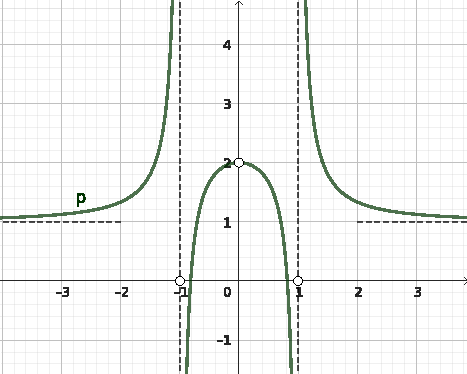
\includegraphics[width=5.0cm]{img/prova-1-nex-função-par-v1.pdf}
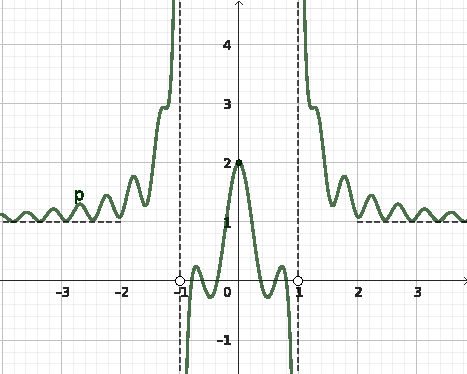
\includegraphics[width=5.0cm]{img/prova-1-nex-função-par-v2.pdf}
\end{center}

\Exercise[title={2,0}] Considerando que $g(x) = \dfrac{2 x^3 - 4 x^2 - 30 x}{-2 x - 6}$, calcule $\displaystyle\lim_{x\to -3} g(x)$ e $\displaystyle\lim_{x\to +\infty} g(x)$.
\Answer Observe que
\[
  g(x)
  = \frac{2 x^3 - 4 x^2 - 30 x}{-2 x - 6}
  = \frac{\cancel{2}x(x^2 - 2 x - 15)}{-\cancel{2} (x + 3)}
  = -\frac{x\cancel{(x + 3)}(x - 5)}{\cancel{x + 3}}
  = -x^2 +5x, \quad \forall x \neq -3.
\]
Então,
\begin{align*}
  \lim_{x\to -3} g(x)
  & = \lim_{x\to -3} -x^2 +5x
    = \left(\lim_{x\to -3} -x^2\right) + \left(\lim_{x\to -3} 5x\right)
    = -\left(\lim_{x\to -3} x^2\right) + 5\left(\lim_{x\to -3} x\right) \\
  & = -(-3)^2 + 5\cdot(-3)
    = -9 - 15
    = -24,
\end{align*}

e
\[
  \lim_{x\to +\infty} g(x)
  = \lim_{x\to +\infty} -x^2 +5x
  = \lim_{x\to +\infty} -x^2
  = -\infty.
\]

\Exercise[title={2,0}] Esboce o gráfico da função $h:\mathbb{R} \to \mathbb{R}$ definida por $h(x) = \begin{cases}
  2-2^{x}&, \text{ se } x < 0\\
  1+\sen(2x) &, \text{ se } x\geq 0,
\end{cases}$
e verifique se existe $\lim_{x\to 0} h(x)$.
\Answer A figura a seguir mostra o gráfico da função $h$:

\begin{center}
  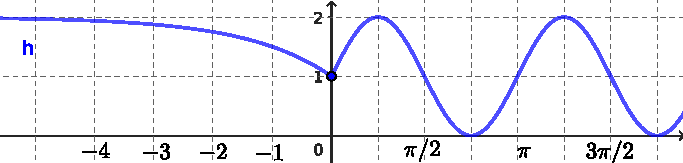
\includegraphics[width=10.0cm]{img/prova-1-nex-função-por-partes.pdf}
\end{center}

Note que para $x < 0$, o gráfico é uma reflexão do gráfico de $y=2^x$ em relação ao eixo $x$ seguida de uma translação de duas unidades para cima. Já para $x \geq 0$, o gráfico é como o da função periódica $y=\sen(x)$, porém ``achatado'' horizontalmente, de modo que seu período é $\pi$ em vez de $2\pi$.

Como a fórmula de $h$ é diferente para $x < 0$ e $x\geq 0$, então devem ser considerados os limites laterais:
\begin{itemize}
  \item $\lim_{x\to 0^-} h(x) = \lim_{x\to 0^-} 2-2^{x} = 2 - 2^0 = 1$
  \item $\lim_{x\to 0^+} h(x) = \lim_{x\to 0^+} 1 + \sen(2x) = 1 + \sen(0) = 1$
\end{itemize}
Já que ambos os limites têm o mesmo valor, conclui-se que $\lim_{x\to 0} h(x)$ existe e também vale $1$.

\Exercise[title={2,0}] Para cada item abaixo, diga se é verdadeiro (V) ou falso (F).

\emph{Observação 1:} Não é necessário justificar.

\emph{Observação 2:} Cada item marcado errado anula a pontuação de um item marcado corretamente. Você tem a opção de deixar o item em branco e, nesse caso, você nem ganha e nem perde pontos.

\begin{enumerate}
  \item {\bf ( \ \ )} \ Para toda função $f$, tem-se $\displaystyle \lim_{x \to 0} \left[ x\cdot f(x) \right] = 0$;
  \item {\bf ( \ \ )} \ $\displaystyle \lim_{x \to 4} \left[ \dfrac{(8 - 2x)^3 - 2 (8 - 2x)}{8 - 2x} - 2x\right]
  = \lim_{u \to 0} \left[ \dfrac{u^3 - 2 u}{u} + \left(u-8\right)\right]$;
  \item {\bf ( \ \ )} \ Sempre que uma função $f$ satisfaz $\displaystyle \lim_{x \to 0} f(x) = 1$ pode-se concluir que $f(0) = 1$;
  \item {\bf ( \ \ )} \ Toda função $g$ que satisfaz $\displaystyle \lim_{x \to -5} g(x) = +\infty$ também satisfaz $\displaystyle \lim_{x \to -5} \dfrac{1}{ g(x) } = 0$.
\end{enumerate}
\Answer

\begin{enumerate}
  \item \textbf{FALSO}: Por exemplo, se $f(x) = \frac{1}{x^3}$, então
  \[
    \lim_{x \to 0} \left[ x\cdot f(x) \right]
    = \lim_{x \to 0} x\cdot \frac{1}{x^3}
    = \lim_{x \to 0} \frac{1}{x^2}
    = +\infty
  \]
  \item \textbf{VERDADEIRO}: Se $u = 8 - 2x$, então $\displaystyle\lim_{x \to 4} u = \lim_{x \to 4} 8-2x = 8-2\cdot 4 = 0$. Além disso, $u-8 = -2x$, e substituindo no limite dado, obtém-se:
  \[
  \lim_{x \to 4} \left[ \dfrac{(8 - 2x)^3 - 2 (8 - 2x)}{8 - 2x} - 2x\right]
  = \lim_{u \to 0} \left[ \dfrac{u^3 - 2 u}{u} + \left(u-8\right)\right]
  \]
  \item \textbf{FALSO}: Uma função pode ter limite em um ponto mesmo sem estar definida no ponto. Por exemplo, $\displaystyle\lim_{x \to 0} \frac{x}{x}= 1$, mas $x=0$ não está no domínio de $f(x) = \frac{x}{x}$.
  \item \textbf{VERDADEIRO}: Considerando a função composta de $f(u) = \frac{1}{u}$ e $u=g(x)$, tem-se
  \[
    \lim_{x \to -5} \dfrac{1}{ g(x) } = \lim_{u \to +\infty} \dfrac{1}{ u } = 0.
  \]
\end{enumerate}
\end{ExerciseList}

\begin{center}
BOA PROVA!
\end{center}

\newpage
\restoregeometry
\section*{Respostas}
\shipoutAnswer
\end{document}
